% arara: xelatex
% arara: nomencl
% arara: xelatex
% arara: indent: { overwrite: yes, trace: yes  }

\documentclass[12pt]{article}


\usepackage[a4paper, top=1in, bottom=1.25in, left=1in, right=1in]{geometry}

\usepackage{amssymb,amsmath}
\usepackage{upgreek} % upright greek symbols

% xetex 西文字体
% https://www.reddit.com/r/typography/comments/2vzkad/a_good_serif_webfont_to_pair_with_fira_sans_thats/
\usepackage{fontspec,xltxtra,xunicode}
    \setmainfont[BoldFont={Charter Bold}, ItalicFont={Charter Italic}]{Charter}
    \setmonofont{Fira Mono}

% 中文字体
\usepackage{xeCJK}
    \setCJKmainfont[BoldFont={Songti SC Bold}, ItalicFont={Kaiti SC Regular}]{Songti SC Regular}
    \xeCJKsetup{CJKecglue = {\hskip 0pt plus 0.08\baselineskip}, xCJKecglue = {false}}
    \punctstyle{plain}

% don't move this line above
\defaultfontfeatures{Mapping=tex-text,Scale=MatchLowercase}

% Line spacing
\linespread{1.5}

% use upquote if available, for straight quotes in verbatim environments
\IfFileExists{upquote.sty}{\usepackage{upquote}}{}
% use microtype if available
\IfFileExists{microtype.sty}{%
    \usepackage{microtype}
    \UseMicrotypeSet[protrusion]{basicmath} % disable protrusion for tt fonts
}{}

\usepackage[unicode=true]{hyperref}
    \urlstyle{same}  % don't use monospace font for urls

\usepackage{graphicx,grffile}
\makeatletter
\def\maxwidth{\ifdim\Gin@nat@width>\linewidth\linewidth\else\Gin@nat@width\fi}
\def\maxheight{\ifdim\Gin@nat@height>\textheight\textheight\else\Gin@nat@height\fi}
\makeatother
% Scale images if necessary, so that they will not overflow the page
% margins by default, and it is still possible to overwrite the defaults
% using explicit options in \includegraphics[width, height, ...]{}
\setkeys{Gin}{width=\maxwidth,height=\maxheight,keepaspectratio}
\IfFileExists{parskip.sty}{%
\usepackage{parskip}
}{% else
\setlength{\parindent}{0pt}
\setlength{\parskip}{6pt plus 2pt minus 1pt}
}
\setlength{\emergencystretch}{3em}  % prevent overfull lines
\providecommand{\tightlist}{%
    \setlength{\itemsep}{0pt}\setlength{\parskip}{0pt}}
\setcounter{secnumdepth}{0}
% Redefines (sub)paragraphs to behave more like sections
\ifx\paragraph\undefined\else
\let\oldparagraph\paragraph
\renewcommand{\paragraph}[1]{\oldparagraph{#1}\mbox{}}
\fi
\ifx\subparagraph\undefined\else
\let\oldsubparagraph\subparagraph
\renewcommand{\subparagraph}[1]{\oldsubparagraph{#1}\mbox{}}
\fi

% set default figure placement to htbp
\makeatletter
\def\fps@figure{htbp}
\makeatother

%%% custom settings

% subcaption
% http://tex.stackexchange.com/questions/125579/subcaption-with-beamer
\usepackage[compatibility=false]{caption}
\usepackage{subcaption}

% for gif
\usepackage{animate}

% chemistry
\usepackage[version=3]{mhchem}
% make inline codes smaller
%\renewenvironment{texttt}{\small}{}
\renewcommand{\texttt}[1]{{\small\ttfamily #1}}

\usepackage{nomencl}
\makenomenclature

\usepackage{etoolbox}


\title{基因系谱与溯祖过程}
\author{Richard R. Hudson \and 许颖 \and 王强}
\providecommand{\institute}[1]{}
\institute{University of Chicago \and 南京大学生命科学学院}

%%% document starts here

\begin{document}
\maketitle

{
    \setcounter{tocdepth}{3}
    \tableofcontents
}

\section{引言}

当比较一组同源 DNA 序列时, 不同序列之间的相似样式包含了这些序列进化历史的信息. 序列数据可以提供多种信息:
哪些序列亲缘关系更近, 不同序列的最近共同祖先出现在多长时间之前. 如果这些序列取自不同的物种,
那么这些信息通常表现为一个推断的系统发生树, 它可能代表了样本物种之间的进化关系. 如果这些序列是取自同一群体内的不同的个体,
而不是取自不同的物种, 那么这些信息就是系谱的, 在此情况下可以推断出基因树. 一个基因树显示了样本序列中哪些序列的亲缘关系更近,
以及这些序列的最近共同祖先出可能出现在什么时候. 一个假想的包含五个序列的样本的基因树或者系谱如图 \ref{fig:1} 所示.
在没有重组的情况下, 每一个序列在上一代有一个单独的祖先. (来自于样本序列的基因树, 与二倍体个体的世系是非常不同的.
每个二倍体个体有两个亲本, 因些向前追溯时祖先的数量会增加.) 现在已经可以获得样本基因的详细系谱信息,
分子群体遗传学的地位也得到了显著的改变.

\begin{figure}
    \centering
    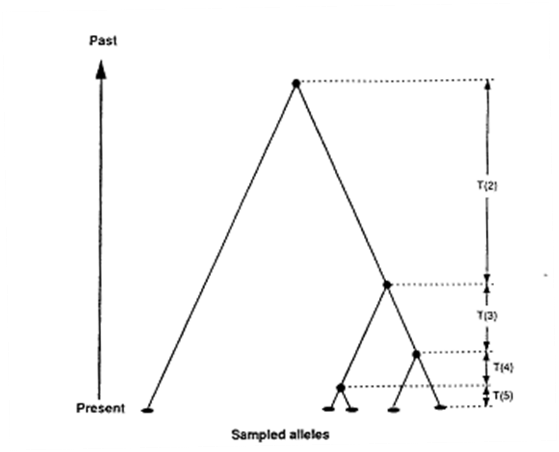
\includegraphics{coalescent-process.images/image1.png}
    \caption{含有五个等位基因的系谱, 显示了溯祖事件间的时间间隔.
        时间间隔 $T(i)$, 用方程 \ref{eq:5} 所给出的期望值成比例的长度表示出来.}
    \label{fig:1}
\end{figure}

在 DNA 时代以前, 分子多态性数据主要是以同功酶频率的形式, 用在凝胶电泳上的迁移率来区分. 通过蛋白电泳,
一个基因的两个同源拷贝可以区分为相同或不同. 如果它们是不同的, 不能衡量有怎样的不同; 如果这两个拷贝是相同的,
我们不能确信它们是真的相同还是某些物理性质的趋同导致了电泳迁移率的相似. 因此,
我们不能从电泳频率的数据中获得基因系谱的细节信息. 运用现代 DNA 技术, 可得到多个个体同源区域的序列,
并且能据此得到关于样本基因系谱的详细信息. Stephens 和 Nei (1985), Aquadro 等 (1986) , Berminghan 和 Avise
(1986), Avise 等 (1987), Cann 等 (1987) 给出了从样本等位基因推断系谱的例子.

对于分子群体遗传学来说, 一个显而易见的挑战就是: 怎样利用这些信息, 来理解影响自然群体中的分子变异的因素. 从理论的角度来说,
基于多个群体遗传学模型, 我们可以从检验那些影响系谱的特性开始. 下面这些问题很重要: 在不同竞争模型下的系谱应该不相同吗?
我们可以设计出不同系谱所需的统计实验吗? 为了把这个任务进行下去, 需要检验样本基因系谱在不同模型下的统计特性.

下文将要阐述, 在多种条件下, 通过分析法或者计算机模拟来推断系谱特性. 这不是关于基因系谱理论的综述, 只是关注无限位点模型的一些看法.
将在中性选择模型下讨论系谱的一些特性, 有或没有重组, 有或没有地理结构, 也会涉及到平衡选择与搭乘效应造成的影响.

下文中也不涉及严密的数学推导处理. 更为精确的推导分析可以在 Kingman (1980,1982a,b) 的论著, Tavare (1984) 的综述,
Griffiths (1980), Watterson (1984) 和 Padmadisatra (1987,1984) 的文章中查阅到.
本文囊括很多了关于等位基因时间的工作 (Donnelly 1986; Donnelly 和 Tavare1986; Tavare 等 1989).
无限等位基因模型和无限位点模型是紧密相关的, 其中一个的结果常常可以用来回答关于另一个的问题. 但是,
这两个模型提出的问题和关心的参数通常是截然不同的. 本文将把注意力集中无限位点模型上,
因为它对于解释群体中的核苷酸多样性是最有用的.

本文将关注于相对小的样本等位基因的性质, 而不考虑关于整个群体的系谱性质的工作, 如固定时间等 (Donnelly 和 Tavare 1987;
Watterson 1982a, 1982b). 并且, 也不会讨论基因树和物种树之间关系 (Hudson 1983b, Neigl 和 Avise 1986; Pamilo
和 Nei 1988; Takahata 1989).

系谱的统计性质强烈依赖于样本的上一代形成下一代的模式. 在本文中, 只讨论 Wright--Fisher (W--F) 模型.
将在下一个小节简要描述此模型中, 上一代产生下一代的模式. 一系列可选择的中性模型本质上有和 W--F 模型相同的系谱性质,
只需要改变时间标度即可 (Kingman 1982a,b; Watterson 1975; Tavare 1984 review; Ewens 1989 review).

\section{不考虑中性突变过程的系谱过程}

本节将详细讨论, 群体大小, 地理结构和选择性保留基因的出现等因素的造成的系谱特性. 系谱特性应该依赖于这些人口统计学因素,
因为实际的系谱依赖于谁有后代而谁没有, 谁迁移了, 迁移去了哪里, 谁的后代含有不普遍的重要突变. 也很明显, 绝对中性的突变 ---
没有和将不会对适合度有影响的突变 --- 应该对随机交配样本的系谱没有影响. 这是因为, 根据定义,
中性突变不影响含有这些突变的个体的后代数或者迁移趋势. 既然这样, 在研究这些系谱性质时就可以不考虑中性突变过程.
所以, 举例来说, 系谱的统计性质不依赖于中性突变是否在迁入者中比在迁出者中更频繁, 或者无限位点,
有限位点还是无限等位基因模型中哪个最合适. 当然, 我们关于系谱过程的推理的统计学性质还是依赖于突变过程. 比如,
如果中性突变的频率很低, 样本中的所有序列可能都是相同的, 就得不到关于样本系谱的信息.

中性突变过程中, 每个后代相对于亲本的突变的位点数符合泊松分布. 突变数的平均值 $\upmu$ 可以假定为常数, 不依赖于基因型,
群体大小和时间. 同时假定突变在不同个体和不同代之间独立发生. 这种突变过程称为恒定突变率的中性突变过程,
也就是标准的中性突变模型 (Kimura 1983; Watterson 1975). 在这些假设下,
沿着世系以不变的方式积累的突变不依赖诸如群体大小, 时间和连锁位点的选择事件等因素. 给定 $t$,
从共同祖先到两个同源样本序列的世代数, $S$, 向下到这两个派生的序列过程中产生的突变数, 是泊松分布的, 有平均值 $2 \upmu
t$. 当 $t$ 是一个随机变量时, 假设是恒定突变率的中性突变过程, 平均数和方差 --- 实际是 $S$ 的所有瞬间值 --- 都是由时刻
$t$ 决定的.

为了强调这一点, 考虑一个群体的某一位点在 0 时刻是完全纯合的, 并且这一位点只发生中性突变. $t$ 代进化之后,
在一个随机取样的个体中检验这一位点. 在我们上一段描述的突变方案之下, 区分我们随机取样的这个个体和 0
时刻时群体中的个体所发生的突变数就是在 $t$ 这段时间内沿着一个特定世系发生的突变数. 突变数是呈泊松分布的, 有平均值 $\upmu
t$. 不论群体大小是多少, 连锁位点是否发生选择, 或者群体是否发生分化. 这是 Birky 和 Walsh (1988)
关于连锁位点发生选择时中性突变积累率的结果的基础. 在以上的例子中, 在 0 到 $t$
时间里固定在整个群体中的突变数要依赖于群体大小和人口统计学方面. 同样地, $t$
时刻群体中的多态性依赖于群体的人口统计学参数, 但是在过去的 $t$ 代的时间里,
沿着某个特定世系发生的突变这使得一个取样的序列不同于它 $t$ 代之前的祖先, 不考虑其他因素, 突变数量是呈泊松分布的, 有平均值
$\upmu t$.

在以下的途径中, 恒定突变率的中性突变过程的作用将会迅速扩大. 令 $T_{\text{tot}}$ 代表一个样本的系谱的所有分支长度的总和.
在上段中讨论的, $S$, 系谱上突变的数量是泊松分布的, 给定 $T_{\text{tot}}$, $S$ 有平均值 $\upmu T_{\text{tot}}$.
一旦 $T_{\text{tot}}$ 的分布在一定的模型下被确定, 很容易得到 $S$ 的分布. 比如说, 如果 $T_{\text{tot}}$
起初的两个时刻能确定, 那么起初的两个时刻的 $S$ 能够根据复合分布的性质计算出来:

\begin{equation} \label{eq:1}
    E(S) = \upmu E(T_{\text{tot}})
\end{equation}

和

\begin{equation} \label{eq:2}
    \text{Var}(S) = \upmu E(T_{\text{tot}}) + \upmu ^{2}\text{Var}(T_{\text{tot}})
\end{equation}

重申, 在我们将要讨论的模型之下, 系谱的性质不依赖于中性突变过程, 因此可以在不准确说明中性突变过程的情况下来研究. 比如说,
我们可以不确定中性突变率或突变模式来研究 $T_{\text{tot}}$ 的统计学性质. 此外,
样本中中性变异的统计性质完全由系谱的统计性质和中性突变过程来决定. 也就是说, 如果两个不同的模型有相同的中性突变过程假设,
并且如果这两个模型有相同的系谱分布, 那么这两个模型的中性变异模式就是相同的. 比如说, 如果中性突变模式如我们前面所描述的,
$S$ 的平均值完全由 $T_{\text{tot}}$ 的平均值决定. 两个不同的模型如果有相同的 $T_{\text{tot}}$ 平均值,
那么就有相同的 $S$ 平均值.

在这一章, 我们会考虑一个理想的单倍体或者二倍体的 W--F 模型. 简言之, 这是一个分离世代的模型, 从单倍体角度, $N$
次取样得到的 $N$ 个子一代单倍体个体 (并且复制可能有突变) 取代亲本一代. 在选择中性的角度, 所有亲代个体有相同可能性作为子代
$N$ 个单倍体个体的亲本. Ewens (1979) 中有这个模型的详细描述. 我们假设 $N$ 很大并且恒定,
在这种情况下个体的后代数目近似于泊松分布. 关于这个模型的大多数结果都是近似的, 和 $(1/N)$ 相比忽略 $(1/N^{2})$ 项.
这和通常对扩散近似所做的假设一致, 称作扩散近似. 与 W--F 模型相比, Moran 模型通常能得到精确结果 (见 Watterson 1975).
这里不讨论 Moran 模型.

\section{最简单的情况: 没有选择也没有重组}

尽管系谱过程在很多已经进行了多年的工作中是不言明的, 但它是关于遗传材料和得到那些激励直接考虑系谱过程的早期工作的序列数据 (或
restriction map 数据) 可能性的本质的知识. Watterson (1975) 引人注目的论文描述了中性模型下系谱的基本性质,
并且标志着现代溯祖理论的开始. 下面关于 W--F 中性模型下非重组系谱的描述大量引自 Watterson (1975), Kingman
(1980,1982a,b), Griffiths (1980) 和 Tajima (1983) 的工作.

首先, 我们考虑一个理想的单倍体物种, 没有重组, 没有地理分化, 没有选择, 一个典型的普通单倍体物种.
我们希望检验从这一群体中随机取样的 $n$ 个个体的系谱性质. 让我们把从群体中取样的时刻标记为 0 代. 从时间上向前回溯 $t$
代的祖先群体称作 $t$ 代.

从这样一个群体中取得的样本的基本性质关系到概率 $P(n)$, $n$ 个取样个体在上一代有截然不同的祖先的概率,
之后的叙述都在这些性质的基础之上. 首先考虑两个个体的样本. 第二个个体和第一个个体有相同亲本的可能性是 $1/N$, 因为在中性
W--F 模型下, 上一代的每一个个体有相同的可能性成为现一代任何一个个体的亲本. 因此 $P(2)$ 是 $1-1/N$.
如果样本含有三个个体, 这三个个体在上一代有不同亲本的可能性就是前两个个体有不同亲本的概率 $\times$
第三个个体和前两个个体没有共同亲本的概率. 有 $N-2$ 个个体是不同于前两个取样个体的亲本的个体,
因此假设前两个个体有不同的亲本, 第三个个体有不同于前两个个体的亲本的概率是 $(N-2)/N=1-2/N$. 总得来说, $n$
个样本个体在上一代有 $n$ 个不同亲本的概率是:

\begin{equation} \label{eq:3}
    P(n) = \prod_{i=1}^{n-1}(1-i/N) \approx 1-\frac{\binom{n}{2}}{N}
\end{equation}

我们可以对 $n$ 个不同的祖先问相同的问题: 它们在前一代有 $n$ 个不同祖先的概率是多少? 很清楚, 还是 $P(n)$. 这意味着 $t$
代之内 $n$ 个样本个体在之前一代有 $n$ 个不同的祖先, 在向前回溯的 $t+1$ 代有两个或更多个体有共同祖先的概率是:

\begin{equation} \label{eq:4}
    P(n)^{t}[1-P(n)] \approx \frac{\binom{n}{2}}{N} e^{-\frac{\binom{n}{2}}{N}t}
\end{equation}

用文字说明就是, 向前追溯到第一个共同祖先出现的时间是呈几何分布的, 并且近似于一个指数分布, 有平均值 $N/\binom{n}{2}$.
对于很大的 $N$ 和很小的 $n$, 如我们通篇假设的, 样本中两个以上个体在同一代里有共同祖先的概率是很小的, 可以被忽略.
因此很可能, 在样本的近期历史中, $t$ 代里存在 $n$ 个不同的世系, 在 $t+1$ 代, 两个样本个体的一对世系溯祖
到了一个最近的共同祖先. 在系谱图上表现为两个世系所代表的分支 ``接合'' 在一个点. 每一个可能的 $\binom{n}{2}$
世系对都有相同的可能性成为找到共同祖先的一对. 继续向前追溯样本的历史, 我们注意在第一次接合的那一代的上一代, 有 $n-1$
个祖先或者说世系可以继续向前追溯. 在每一代中所有祖先在上一代有不同祖先的可能性是 $P(n-1)$.
所以到下一次接合的时间近似指数分布, 平均值是 $N/\binom{n-1}{2}$. 在这个接合, 每一个可能的 $\binom{n-1}{2}$
世系对都有相同的可能性在这一点接合. 注意, $(n-1)$ 个世系中的一个在我们起初的样本中有两个后裔, 其他的世系有一个.
我们可以按照这种方式继续下去, 直到所有世系接合到一个世系, 样本里全部的 $n$ 个个体的共同祖先.

如图 \ref{fig:1} 中所示的五个样本等位基因的系谱. 产生一个谱系的随机过程, 被称为溯祖过程, 可以简要概括出来. 时间
$T(j)$, 有 $j$ 个不同世系的时间近似呈指数分布, 如果以 $N$ 代为单位衡量时间, $T(j)$ 的平均值是:

\begin{equation} \label{eq:5}
    E[T(j)]=\frac{1}{\binom{j}{2}}
\end{equation}

在 $t$ 代所有世系中随机选择的两个世系在 $t+1$ 代接合在系谱图的一个节点. 注意, 我们没有关心我们样本的祖先之外的世系.
也要注意, 接合之间的时间间隔 $T(j)$ 互不依赖. 并且, 需要指出系谱图上老的部分 (图 \ref{fig:1} 中系谱图的上一部分)
与小样本系谱图在统计学性质上是相同的. 比如说, 样本数为 $n$
的样本的历史中系谱图上第一个最近共同祖先以上部分的分布与样本数为 $n-1$ 的样本是完全相同的.
在计算机中生成这样的系谱是没有意义的. (附录中给出了一个程序的例子) .

这些系谱性质可以用于普通的单倍体生物, 也可以用于线粒体基因组. 如果线粒体遗传是严格母系的并且母本个体内的多态性是可以忽略的,
$N$ 的值就是母本的数目.

对于 $N$ 个二倍体个体的大群体, 在随机交配的 W--F 模型下, 没有重组和选择, 结果也是一样, 只是要用 $2N$ 代替 $N$.
这种情况下, 系谱应该被想成是没有重组的特定位点的系谱. 这些位点可能含有一个核苷酸位点, 或者, 如果重组率十分低,
很多可以认为是完全连锁的相邻核苷酸位点. 按照正在考虑的模型, 十分低意味着 $Nr\ll 1$, 其中 $r$
是每一代所关心的区域两端之间的重组率. 如果在单倍体模型中以 $N$ 代为单位衡量时间, 在二倍体模型中以 $2N$ 代为单位衡量时间,
单倍体和二倍体的结果是完全相同的, 即 $T(j)$ 由方程 \ref{eq:5} 给出.

在大的群体中不连锁的位点在本质上是独立的, 有各自独立的系谱. 连锁的位点, 有相关的系谱, 之后会考虑到.

\section{系谱中加入中性突变}

假设有我们刚刚讨论的系谱性质, 我们可以预言各种各样突变下的样本的性质. 如之前部分所讨论的,
我们假设一个恒定突变率的中性突变过程, 其中每一个子代配子相对于亲本的突变个数平均值为 $\upmu$. 另外,
我们假设一个无限位点模型 (Kimura 1969). 在这个模型下, 基因座由很多位点组成,
所以在我们的样本系谱中每个位点发生的突变不多于 1 个. 没有采用的无限等位基因模型 (Kimura 和 Crow 1964) 是相似的,
假设每个突变产生一个不存在于样本系谱其他任何地方的新基因. 对于我们的目的, 无限等位基因模型和无限位点模型在本质上是相同的,
但是在无限等位基因模型下会忽略多少个突变区分等位基因, 并且只注意到等位基因是否相同.

我们关心的首要性质是关于发生在一个样本的系谱分支上的突变的个数的分布. 在无限位点模型下,
突变的个数和样本中有多态性的核苷酸位点的数目是相同的. $S$ 代表样本中多态性位点的数目, 常常被说成是样本中的分离位点
(segregating sites). 首先, 我们考虑 $S$ 的期望值.

从方程 \ref{eq:1} 我们可以从系谱的总长度 $T_{\text{tot}}$ 的期望计算 $S$ 的期望. 从 $T(j)$
的定义很容易知道系谱分支的总长度是 $\sum_{i=2}^{n} i T(i)$. 因此, 以 $2N$ 为单位衡量时间, 从方程
\ref{eq:5} 可得到:

\begin{equation} \label{eq:6}
    E(S)=\frac{\uptheta}{2} \sum_{i=2}^{n} iE(T(i)) = \uptheta \sum_{i=1}^{n-1}1/i
\end{equation}

其中 $\uptheta = 4N \upmu$ (Watterson 1975). 总时间的方差也很容易得到, 用方程 \ref{eq:2} 和 \ref{eq:6}, 得到
(Watterson 1975):

\begin{equation} \label{eq:7}
    \text{Var}(S) = \uptheta \sum_{i=1}^{n-1} \frac{1}{i} + \uptheta^{2} \sum_{i=1}^{n-1} \frac{1}{i^{2}}
\end{equation}

实际上, 任何时刻的 $S$ 都可以用这一时刻的 $T_{i}$ 的形式表示. Watterson
证明了分离位点的数目在足够大小的样本中是近似正态分布的.

我们可以得到 $S$ 的总体分布, 但是首先我们考虑 2 个个体的样本 $S=0$ 的概率. 这和纯合的期望 $E(F)$ 是相等的,
或者这两个样本基因相同的概率. 这个概率可以从两个途径得到. 如果在无限位点模型 (或无限等位基因模型) 下两个样本基因是相同的,
就必须是在从最近共同祖先 (可用 MRCA 表示) 向下到它们的世系上没有发生突变的情况下. 假定 $t$
为回溯到它们的共同祖先的世代数, 从 MRCA 向下过程中没有发生突变的概率是 $\mathrm{e}^{-2\upmu t}$.
这从突变的泊松假设可以得到. 因此, 如果我们得到期望 $\mathrm{e}^{-2\upmu t}$, 在 $t$ 的分布之上, 我们得到:

\begin{equation} \label{eq:8}
    E(F) = E(\mathrm{e}^{-2\upmu t}) = \int_{0}^{\infty} \frac{\mathrm{e}^{-\frac{t}{2N}}}{2N}\mathrm{e}^{-2\upmu t} dt = \frac{1}{1+\uptheta}
\end{equation}

$t$ 是指数分布的, 在二倍体模型中有平均值 $2N$.

这是一个经典结果 (Kimura 和 Crow 1964), 当然可以用递归方法得到, 但是在这里需要知道它和系谱的联系.

方程 \ref{eq:8} 也举例说明了无限等位基因模型和溯祖过程之间的联系. 对于群体过程的任何一个决定系谱过程的模型,
如果突变过程是我们已经假设的无限等位基因恒定突变率中性突变过程, 两个随机取样的等位基因相同的概率是 $C(\uptheta
)=E(\mathrm{e}^{-\uptheta t})$, 其期望和 $t$ 的分布有关, $t$ 是以 $2N$ 代为单位衡量的两个随机等位基因回溯到 MRCA
的时间. 相同性系数以 $-\uptheta$ 为参数, $C(-\uptheta )$ 也是 $t$ 的矩量母函数 (moment generating function) .
瞬时的 $t$ 以及相应的瞬时 $S$ , 很容易用标准方法从 $C(\uptheta )$ 得到. 比如说, $E(t)$ 是 $–C'(0)$, $E(S)$ 是
$–\uptheta C'(0)$, 其中 $–C'(0)$ 代表 $-C(\uptheta )$ 的导数, 取 $\uptheta = 0$. 这很一般的. 比如说,
在多基因家族中保守的基因模型下, 一对取样的等位基因的相同性系数已经从多种途径得到 (Nagylaki 和 Petes 1982) .
只要用相同性系数的导数来描述, 在无限位点模型下区分这些等位基因的瞬时位点数目就可以计算.

方程 \ref{eq:8} 的一个导数包括两个取样基因在时间上向前追溯的历史, 直到找到这两个等位基因的 MRCA
或者找到了其中一个世系上的一个突变. 在每代, MRCA 出现的概率 $P_{\text{CA}}$ 是 $1/2N$. 同样, 在每一代,
两个世系中的某一个发生突变的概率 $P_{\text{mut}}$ 是 $2\upmu$. 当且仅当先遇到的时间是一个共同祖先时,
这两个等位基因才可能相同. 假定这两个事件中的某一个发生了, 并且忽略这两个事件在同一代发生的概率,
先遇到的事件是共同祖先的概率是:

\begin{equation} \label{eq:9}
    E(F) \approx \frac{P_{\text{CA}}}{P_{\text{CA}}+P_{\text{mut}}}=\frac{1/2N}{1/2N+2\upmu }=\frac{1}{1+\uptheta }
\end{equation}

同样的方式, 可以得到 2 个个体的样本到共同祖先所发生的突变数目的总体分布. $P_{2}(j)$, 从 MRCA 开始 $j$
个突变发生在世系上的概率, 就是起初的 $j$ 个事件是突变、第 $(j+1)$ 个事件是一个共同祖先的概率. 因此, 我们有
(Watterson, 1975):

\begin{equation} \label{eq:10}
    P_{2}(j)=\left (\frac{\uptheta}{1+\uptheta}\right )^{j}\frac{1}{1+\uptheta}
\end{equation}

用同样的理由, 我们可以得到有 $n$ 个祖先世系时发生 $j$ 个突变的概率 $Q_{n}(j)$. 得到 $j$ 个突变的这段时间, 有 $n$
个世系, 前 $j$ 个事件必须是突变, 第 $(j+1)$ 个事件必须是共同祖先. 因此, 概率是:

\begin{equation} \label{eq:11}
    \begin{split}
        Q_{n}(j) & = \left (\frac{n\upmu}{n\upmu + \frac{\binom{n}{2}}{2N}} \right )^{j} \frac{\frac{\binom{n}{2}}{2N}}{n\upmu + \frac{\binom{n}{2}}{2N}} \\
        & = \left (\frac{\uptheta}{\uptheta + n - 1} \right )^{j} \frac{n-1}{\uptheta + n - 1}
    \end{split}
\end{equation}

大小为 $n$ 的样本中分离位点的数目是 $n$ 个世系时发生的个数和系谱中剩余部分发生个数的加和, 在其他部分的分布如同一个大小为
$n-1$ 的样本. 大小为 $n$ 的样本中有 $j$ 个分离位点的概率 $P_{n}(j)$ 可以写作:

\begin{equation} \label{eq:12}
    P_{n}(j) = \sum_{i=0}^{j} P_{n-1}(j-1) Q_{n}(i)
\end{equation}

分离位点个数的分布可以用这个递归公式很快计算出来. Tavare (1984) 得到了 $P_{n}(j)$ 的一个明确的表达式. 图
\ref{fig:2} 显示了 $\uptheta=5$ 和 $n=20$ 的 $S$ 的分布.

\begin{figure}
    \centering
    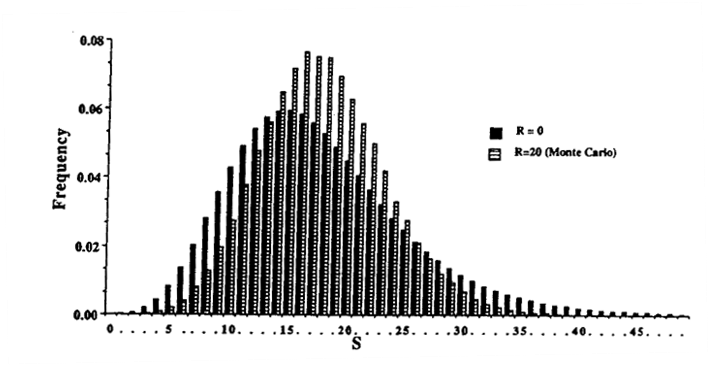
\includegraphics{coalescent-process.images/image2.png}
    \caption{在一个含有 20 个等位基因 $\uptheta = 4N\upmu = 20$ 的样本中分离位点数 $S$ 的分布.
        用方程 \ref{eq:12} 计算无重组 (no-recombination) 分布 ($\mathrm{R}=4N\upmu =0$).
        对于 $R=20$, 分布是用文中所述的蒙特卡洛方法做 100000 个重复得到的一个估计.
        两种分布中 $S$ 的期望值都是 17.7, 这个值可以用方程 \ref{eq:6} 计算出来.}
    \label{fig:2}
\end{figure}

下面的例子说明了方程 \ref{eq:12} 的应用. 在最近一个果蝇黄色--无刚毛--鳞甲区域 (yellow--achaete--scute region of
\textit{Drosophila melanogaster}) 中多态性的调查中, 在所调查的 64 个染色体上的 2112 个核苷酸位点中发现了 9
个多态性位点 (Aguade et al. 1989). 从果蝇染色体组的其他区域估算每个碱基对的 $\uptheta$ ($\uptheta$ per base
pair) 有平均值 0.005. Aguade 等想确定 9 个多态性位点的观察值是否符合黄色--无刚毛--鳞甲区域每个碱基对的 $\uptheta$
是 0.005. 用方程 \ref{eq:12} , 我们可以计算 9 个或更小的多态性的概率, 在一个大小为 64 的样本中, $\uptheta =
2112(0.005) = 10.6$, 概率近似为 $2 \times 10^{-6}$. 假设中性平衡理论是正确的, 必须拒绝 0.005
作为这一区域的每个碱基对的突变参数值. 如果假设在这一区域发生了重组, 9 个多态性位点或更少的概率会更小.

\section{重组}

让我们先考虑两个基因座. 假设这两个基因座之间没有发生重组, 但是每一代每产生一个后代, 重组的可能性是 $r$. 如果 $r=0$,
那么这两个基因座永远有同样的系谱. 如果 $r$ 很大, 在一个大的随机交配群体中, 这两个基因座的系谱终将会是独立的 (见方程 13).
困难的情况是系谱在这两个基因座相关 (are correlated) 时, 有中间水平的重组. 显然,
中型模型下每个基因座的系谱的边缘分布是上文所述的没有重组的单个位点的分布. 连锁的唯一作用是制造了两个基因座的系谱之间的联系
(correlation) .

让我们从描述如何在计算机上模拟一个两配子样本的系谱开始, 用 $\mathbf{a}_{1}(0)\mathbf{b}_{1}(0)$ 和
$\mathbf{a}_{2}(0)\mathbf{b}_{2}(0)$ 表示. 我们像之前一样, 沿时间向前追溯. 我们向前追溯这两个世系直到一个共同祖先
(coalescent) 出现 (每一代的可能性是 $1/2N$) 或者一个重组事件出现 (每一代的可能性是 $2r$) .
追溯至其中一个事件发生的时间是指数分布的, 有平均值 $2N/(1+R)$, 其中 $R$ 是 $4Nr$.
首先发生的事件是一个溯祖事件的可能性是 $1/(1+R)$. 在这种情况下, 这两个位点这时有了 MRCA, 并且系谱完整.
另一种可能性是首先发生的事件是一个重组事件. 首先发生的事件是重组事件的可能性是 $R/(1+R)$. 在这种情况下,
这两个世系中的一个分裂成两个, 如图 3 的系谱所举例说明的. 在这个例子中, 沿时间向前追溯, 第一个的事件是发生在 $t_{1}$
代的重组. 在这个例子中, 祖先配子, $\mathbf{a}_{2}(t_{1}-1)\mathbf{b}_{2}(t_{1}-1)$, 是 $t_{1}$
代的两个个体的重组后代, 用 $\mathbf{a}_{2}(t_{1})\text{-}$ 和 $\text{-}\mathbf{b}_{2}(t_{1})$ 表示.
在这个点, $t_{1}$ 代中有三个世系要从这三个祖先配子向前追溯. 一个祖先配子, 用
$\mathbf{a}_{1}(t_{1})\mathbf{b}_{1}(t_{1})$ 表示, 在这两个位点上都是其中一个样本配子的祖先. 其中一个祖先配子,
用 $\mathbf{a}_{2}(t_{1})\text{-}$ 表示, 是样本中 $\mathbf{a}_{2}$ 基因的一个祖先, 但是这个祖先配子的
$\mathbf{b}$ 基因, 用一个连字符表示的, 在样本中没有后代. 用连字符代表的这个基因的历史没有直接的兴趣. 第三个祖先配子,
$\text{-}\mathbf{b}_{2}(t_{1})$, 是样本中的 $\mathbf{b}_{2}$ 基因在 $\mathbf{b}$ 位点上的祖先.
我们继续沿时间向前追溯直到下一个事件, 这三个世系中的任意两个之间找到共同祖先 (每一代的可能性是 $\binom{3}{2}/2N$
或者一个重组事件 (每一代的可能性是 $r$) . 注意, 在系谱的这个部分中, 只有包含
$\mathbf{a}_{1}(t_{1})\mathbf{b}_{1}(t_{1})$ 世系的重组是有关的. $\mathbf{a}_{2}(t_{1})\text{-}$
世系中的重组不会造成这个过程的任何改变, 与样本等位基因的系谱没有关系. 最终, $\mathbf{a}$
位点上的两个等位基因会找到一个共同祖先, $\mathbf{b}$ 位点上的两个等位基因会找到一个共同祖先,
这样这个两位点的系谱就完整了.

\begin{figure}
    \centering
    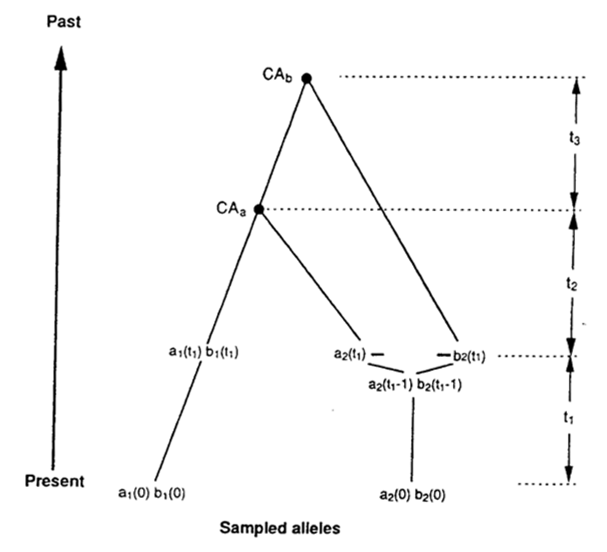
\includegraphics{coalescent-process.images/image3.png}
    \caption{大小为 2 的一个样本的两基因座系谱举例. 其中, 第一个事件是发生在 $t_{1}$ 代的一个重组事件, 祖先配子
        $\mathbf{a}_{2}(t_{1}-1)\mathbf{b}_{2}(t_{1}-1)$ 是 $t_{1}$ 代的 $\mathbf{a}_{2}(t_{1})\text{-}$ 和
        $\text{-}\mathbf{b}_{2}(t_{1})$ 两个配子的重组后代. 第二个事件是一个共同祖先事件, 用 $\text{CA}_{\mathbf{a}}$
        标记, 在这个时间点, 世系 $\mathbf{a}_{1}(0)\mathbf{b}_{1}(0)$ 和 $\mathbf{a}_{2}(t_{1})\text{-}$
        找到最近共同祖先. 就是在这个时间点, $t_{1}+t_{2}$ 代之前. 取样的 $\mathbf{a}$ 基因座等位基因的最近共同祖先出现了.
        下一个事件是一个共同祖先事件, 用 $\text{CA}_{\mathbf{b}}$ 标记. 这时, $t_{1}+t_{2}+t_{3}$ 代之前, 取样的
        $\mathbf{b}$ 基因座等位基因的最近共同祖先出现了.}
    \label{fig:3}
\end{figure}

\begin{figure}
    \centering
    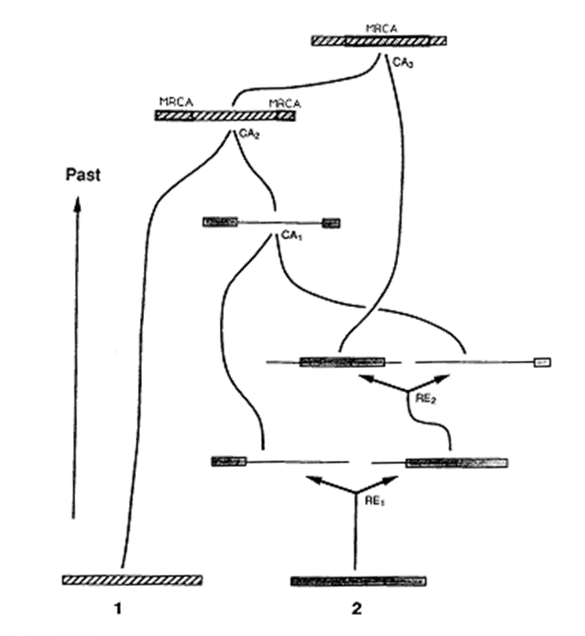
\includegraphics{coalescent-process.images/image4.png}
    \caption{无限位点重组模型的系谱举例. 用 1 和 2 标记的两个样本配子用阴影线和点状的条表示. 重组事件可以在条的任何位置发生.
        系谱上有五个事件, 按照从现在到古代的顺序, 西系谱上有五个事件, 用 $\text{RE}_{1}$, $\text{RE}_{2}$,
        $\text{CA}_{1}$, $\text{CA}_{2}$ 和 $\text{CA}_{3}$ 表示. 最近的事件, $\text{RE}_{1}$ 是一个重组事件,
        把两个片段带到一起形成配子 2 的祖先. 像往常一样, 从时间上向前追溯的之后世系, $\text{RE}_{1}$ 的结果是配子 2
        的世系分裂成两部分, 一个是左边终于这个配子的世系, 另一个是配子右边部分的世系. 系谱上的下一个事件, 用 $\text{RE}_{2}$
        标记, 也是一个重组事件, 配子 2 祖先的右侧片段有一个转型. 在这个时间点上, 有三个不同的配子 2 的祖先, 每一个都是配子 2
        不同部分的祖先. 相比之下, 配子 1 有一个单独的祖先. 下一个事件, $\text{CA}_{1}$ 是一个共同祖先事件, 涉及到配子 2
        的两个祖先. 在这一点, 配子 2 的两个祖先中的一个是配子 2 的两个不相邻部分的祖先. 下一个事件, $\text{CA}_{2}$
        是一个共同祖先事件, 配子 1 和 2 的一部分的最近共同祖先终于出现. 在这一点有最近共同的片段是左边末端, 用 MRCA 标记的,
    和右边末端, 也用 MRCA 标记. 最后一个事件, 是一个共同祖先事件, 样本配子中间片段的最近共同祖先出现.}
    \label{fig:4}
\end{figure}

考虑这个两基因座过程, 可能得到时间的联合分布 (joint distribution) 的多种性质, $t_{\mathbf{a}}$ 和
$t_{\mathbf{b}}$, 代表回溯到 $\mathbf{a}$ 和 $\mathbf{b}$ 基因各自的最近共同祖先的时间.

Griffiths (1981a) 得到了大小为 2 的样本中每个基因座的分离位点数目的联合分布的性质,
前提是每个基因座都假设是无限位点基因座. 从 Griffiths 的结果, $t_{\mathbf{a}}$ 和 $t_{\mathbf{b}}$, 即
$\mathbf{a}$ 基因座和 $\mathbf{b}$ 基因座到 MRCA 的时间, 之间的关系可以找到 (Hudson 1983a; Kaplan 和 Hudson
1985):

\begin{equation} \label{eq:13}
    \text{Cor}(t_{\mathrm{a}},t_{\mathrm{b}})=\frac{R+18}{R^{2}+13\mathrm{R}+18}
\end{equation}

对这两个基因座溯祖的考虑, 显示了 $t_{\mathbf{a}}=t_{\mathbf{b}}$ 的可能性和 $t_{\mathbf{a}}$ 间
$t_{\mathbf{b}}$ 的关系完全相同 (Hudson, 未发表) .

Hedrick 和 Thomson 把基于两基因座溯祖的模拟用于研究中性模型的两基因座样本性质. Kaplan 和 Hudson (1985)
关注了几个连锁基因座的溯祖过程, 计算了由几个之间可能发生重组的亚基因座 (sub-loci) 组成的总的基因座上的纯合性.

Hudson (1983a) 和 Kaplan 和 Hudson (1985) 也关注了以上溯祖过程的无限位点形式,
在无限位点模型中重组可以发生在任何一个代表一个紧邻核苷酸位点的延伸的连续间隔上. 图 4
显示了一个这个模型下的两配子样本系谱的代表. 这个过程与先前的两基因座情况非常相似, 除了重组在沿着代表序列 (represcent the
sequence) 的连续间隔的随机位置发生 (我想, 意思是重组的位置随机) . 在这种情况中, 小的相邻片段可能有相似的系谱,
但是相距较远的片段可能有很不相同的系谱. Hudson (1983a) 描述了怎样实现这样一个模拟的细节.

在图 4 的系谱中, 与处在末端的片段相比, 处于中间的 DNA 片段的 MRCA 在时间上向前追溯得更远. 在这层意义上,
中间片段的系谱的尺寸比末端片段要大, 并且假设片段上各处的中性突变率相同, 我们可以假设中间片段上每个单位长度的突变个数更多.
在图 5 中, 显示了一个容量为 10 的样本中大量临近的 DNA 系谱过程的一个深入了解的结果. 这个图指出了系谱的大小 (size)
有多大, 用 $T_{\text{tot}}$ 来衡量, 一个片段可能不同于下一个. 在图 5 中考虑的 DNA 片段大小是这样: $4Nr$ 等于 100, 其中
$r$ 是区域末端之间每代的重组率. 尽管这种估计非常粗略, 已经估计符合 \textit{D. melanogaster} 中的大约 5000 bp.
(这个数字可以从每个碱基重组率为 $0.5\times 10^{-8}$ 和有效种群大小为 $10^{6}$ 的估计中得到:  (Hudson 和 Kaplan
1988; Hudson 1987.)

如之前所说, 样本中分离位点的总数, $S$, 依赖所有片段的系谱, 呈泊松分布, 平均值为 $\uptheta T/2$, 在这种情况下 $T$
是每个依靠它们的长度加权的片段的系谱的平均大小, 并且 $\uptheta$ 是整个序列突变率的 $4N$ 倍. 随着重组率的增加, 加权平均值
$T$ 由更多数量的相对较小的那些拥有关联较少的系谱的片段组成. 结果是 $T$ 的方差 (变异数? variance) 趋向于 0, 并且 $S$
成为泊松分布, 同时重组系数 ($R$) 趋向无穷 (见 Ewens 1979, p.276) . Kaplan 和 Hudson (1985) 表明了 $S$
的方差为:

\begin{equation} \label{eq:14}
    \text{Var}(S) \approx \uptheta \left(\overset{n-1}{\underset{i=1}\sum }1/i \right) + \uptheta ^{2}\text{Var}(T)
\end{equation}

并且

\begin{equation} \label{eq:15}
    \begin{split}
        \text{Var}(T) & \approx \frac{2 \left(\sum_{i=1}^{n-1} 1/i \right)}{R^{2}}(-R \\
        & + \frac{23R+101}{2\sqrt{97}} \log \left(\frac{2R+13-\sqrt{97}}{2R+13+\sqrt{97}} \frac{13+\sqrt{97}}{13-\sqrt{97}} \right) \\
        & + \frac{R-5}{2}\log \left(\frac{R^{2}+13R+18}{18} \right))
    \end{split}
\end{equation}

对于容量为 2 的样本, $\text{Var}(T)$ 的近似值是建立在通常的 ``扩散近似值'' 的基础之上的, 但是对于大的样本容量,
近似值没有理论上在正当理由, 除了蒙特卡洛模拟显示它在这个检验过的情况下非常有效, 也就是小范围修正 $R$ 值 (namely with
small to moderate values of $R$) (Kaplan 和 Hudson 1985) . Hudson 和 Kaplan (1985)
已经检验了样本系谱中重组事件的数量, 得到了基于事件推断数量之上的 $R$ 的估计值. 当包含这两个位点的四个可能的配子类型
(单倍体型) 出现在样本中时, 可以推测两个多态性位点之间已经发生重组.

\begin{figure}
    \centering
    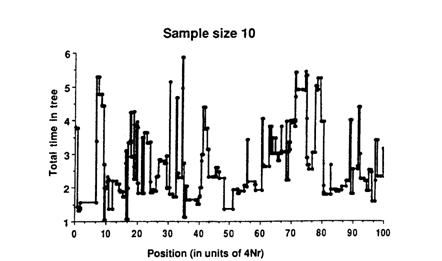
\includegraphics{coalescent-process.images/image5.png}
    \caption{样本系谱上的总时间, $T_{\text{tot}}$, 以 $4N$ 代为单位衡量, 写成位置的函数,
        对于中性无限突变位点重组模型的溯祖过程的一个单独 realization. 所考虑的 DNA 区域的总长度是 $4Nr=100$, 其中 $r$
        是区域末端之间的重组率. 水平轴式核苷酸位置, 用 $4N$ 的结果和这个位点与所考虑的区域的左侧末端间的重组率来衡量. 显然,
        在这样大小的一个区域上, 各个位点的 $T_{\text{tot}}$ 有相当大的不同.}
    \label{fig:5}
\end{figure}

图 \ref{fig:2} 显示了容量为 20 的样本中 $S$ 的分布, 其中 $\uptheta =5$, $R=0$ 和 $R=20$. $S$ 的平均值不依赖于
$R$, 但是这张图清楚地显示了重组怎样减小了 $S$ 的方差. 这个显示了 $R=20$ 的分布是以用上述运算法则生成的 100000
个样本为基础的. $S$ 在蒙特卡洛样本中的方差是 28.04, 而用方程 (14) 和 (15) 计算出来的方差是 28.28.

\section{估算 $\uptheta$ 或 $N$}

群体大小为 $N$, 如果已知中性突变率 $\upmu$, 可以用 $S$ 估算 $\uptheta$. 两种常用的方法是瞬时估计.
因为两个等位基因之间期望值的差别是 $\uptheta$, $\uptheta$ 的观察量是 $\overset{‾}{\uptheta}$,
样本中等位基因之间差别数的平均对数 (见 Nei 1987, 方程 10.6). 这是 $\uptheta$ 的一个无偏性估计量. Tajima (1983) 说明了在
W--F 模型下无重组时, 估计量的方差是 (见 Nei 1987 方程 10.9):

\begin{equation} \label{eq:16}
    \text{Var}(\hat{\uptheta})=\frac{n+1}{3(n-1)}\uptheta + \frac{2(n^{2}+n+3)}{9n(n-1)}\uptheta^{2}
\end{equation}

Watterson (1975)在方程 (6) 的基础上提出了一个估计量, 即:

\begin{equation} \label{eq:17}
    \hat{\uptheta}=\frac{S}{\sum_{i=1}^{n-1}1/i}
\end{equation}

这个估计量明显是无偏性的. 在无重组的模型下, 这个估计量的方差容易用方程 (7) 计算出来, 因为:

\begin{equation} \label{eq:18}
    \text{Var}(\hat{\uptheta})=\frac{\text{Var}(S)}{\left( \sum_{i=1}^{n-1} 1/i \right)^{2}}
\end{equation}

$\uptheta$ 的方差总小于 $\overset{‾}{\uptheta}$ 的方差. 在有重组的情况下, 这两个估计量的方差都显著减小.
在有重组的情况下, $\hat{\uptheta}$ 的方差可以用公式 (14) , (15) 和 (18) 来估算.

在一些情况下, 有重组时 $S$ 方差的减小可能是某些问题中考虑核基因代替线粒体基因的理由. 比如说, 最近的线粒体基因组研究
(Avise 等 1988)用于估算有效群体大小, 用先前的 $\upmu$ 的估计. 尽管和核基因相比, 出于 mtDNA
相对容易分离的考虑对核基因的应用不利, 但是更多准确的估算可能从核数据获得.

对于没有重组的模型, 基于 $S$ 的 $\uptheta$ 的最大可能性估算能够获得, 并且能证明最大可能性估计总是超过 $\hat{\uptheta}$
(Tavare 1984). Hudson 检验了少数几种情况, 并且总能发现最大可能性估计的方均误差总是超过 $\hat{\uptheta}$ 的方均误差.

\section{迁移和地理结构}

当存在地理结构时, 许多作者已经利用系谱途径去考虑样本性质 (Griffiths 1981b; Slakin 1987, 1989; Strobeck 1987;
Tajima 1989, Takahata 1988). 为了举例说明这些原则, 我们考虑一个两群体对称岛模型 (two-population symmetric
island model). 每个亚群体由 $N$ 个二倍体组成. 每一代, 每个亚群体的一个小部分 $m$ 是由来自另一个亚群体的移民构成.
换句话说, 每个个体的亲本是定居在相同群体中的概率是 $1-m$, 在另一个亚群体中的概率是 $m$. 根据 panmictic 模型,
来自同一亚群体的两个等位基因在上一代有一个共同祖先的概率是 $1/2N$.
来着不同亚群体的两个等位基因在上一代有共同祖先的概率可以忽略. 把这些性质放在一起, 我们可以描述包含 $n$
个等位基因的样本的系谱过程, 其中 $n_{1}$ 个来自亚群体 1, $n_{2}$ 个来自亚群体 2. 我们用有序偶 (order pair),
$(i,j)$, 表示祖先世系的情况, 表示 $i$ 个祖先在亚群体 1 中而 $j$ 个在亚群体 2 中. 像往常一样,
我们在时间上向前追溯世系, 直到出现一个共同祖先或者其中一个世系改变定居亚群体. 这个时间是指数分布的, 有平均值

\begin{equation*}
    \frac{1}{(\binom{n_1}{2}+\binom{n_2}{2}+(n_{1}+n_{2})\frac{M}{2})}
\end{equation*}

以 $2N$ 代为单位衡量时间, 并且其中 $M=4Nm$. 假设这两个事件中的一个发生, 是亚群体 $i$ 中 $n_{i}$
个世系中的一个共同祖先的概率是:

\begin{equation*}
    \frac{\binom{n_i}{2}}{(\binom{n_1}{2}+\binom{n_2}{2}+(n_{1}+n_{2})\frac{M}{2})}
\end{equation*}

如果共同祖先事件发生在亚群体 1 中, 祖先世系的情况变成 $(n_{1}-1,n_{2})$. 这个事件是亚群体 $i$
中的一个世系住处改变的概率是:

\begin{equation*}
    \frac{n_{i}\frac{M}{2}}{(\binom{n_1}{2} + \binom{n_2}{2} + (n_{1}+n_{2})\frac{M}{2})}
\end{equation*}

如果一个世系从亚群体 1 中改变到亚群体 2 中, 沿时间向前追溯仍然有效, 祖先世系的情况变成 $(n_{1}-1,n_{2}+1)$.
这个过程可以继续.

如上所述, 这个过程可以进行蒙特卡洛模拟. Strobeck (1987), Tajima (1989)和 Slatkin 和
Maddison(1989)已经实现了基于这个途径的蒙特卡洛模拟.

为了举例证明怎样通过这个途径得到分析的结果, 我们计算从同一个亚群体中取样得到两个等位基因相同的概率, $P_{s}(theta )$,
和来自不同亚群体的两个等位基因相同的概率, $P_{d}(theta )$. 如前面说的, 一旦得到这些相同性系数, 我们可以计算瞬时的 $S$.
前面我们假设了一个对称岛模型, 除了是用 $n$ 个亚群体. 我们沿时间向前追溯来自同一个亚群体的两个等位基因的系谱,
直到一个共同祖先、突变或者迁移事件出现. 如果第一个事件是一个共同祖先事件, 概率是 $1/(1+theta +M)$,
这两个等位基因是相同的. 如果第一个事件是一个突变事件. 概率是 $\uptheta /(1+theta +M)$, 这两个等位基因是不同的.
如果第一个事件是迁移, 这两个等位基因相同的概率是 $P_{d}(theta )$. 从此可以导出以下 $P_{s}(theta )$ 的方程:

\begin{equation} \label{eq:19}
    P_{s}(\uptheta)=\frac{1}{1+\uptheta +M}\cdot 1+\frac{\uptheta}{1+\uptheta +M}\cdot 0+\frac{M}{1+\uptheta +M}P_{d}(\uptheta)
\end{equation}

对于两个来自不同群体的等位基因, 只有把两个世系带入同一个亚种群的突变和迁移事件需要考虑. 如果第一个事件是一个突变事件,
概率为 $\uptheta /(\uptheta +M/n)$, 这两个等位基因是不同的. 如果第一个事件是把一个世系带入另一个亚种群的迁移事件, 概率为
$(M/n)/(\uptheta +M/n)$, 相同的概率为 $P_{s}(\uptheta)$. 由此可以导出以下 $P_{d}(\uptheta)$ 的方程:

\begin{equation} \label{eq:20}
    P_{d}(\uptheta)=\frac{\frac{M}{n}}{\uptheta +\frac{M}{n}}P_{s}(\uptheta)
\end{equation}

解方程 (19) 和 (20) ,

\begin{equation} \label{eq:21}
    P_{s}(\uptheta)=\frac{(n-1)\uptheta +M}{(n-1)\uptheta ^{2}+\uptheta (n-1+Mn)+M}
\end{equation}

并且

\begin{equation} \label{eq:22}
    P_{d}(\uptheta)=\frac{M}{(n-1)\uptheta ^{2}+\uptheta (n-1+Mn)+M}
\end{equation}

这些结果不是新的, 其他人已经得到过, 没有考虑溯祖过程 (见 Crow 和 Aoki, 1984, 和其中的参考文献) .
为了得到到达共同祖先的时间的期望值, $t_{s}$ 和 $t_{d}$, 分别代表这两个等位基因来自相同亚群体和不同亚群体,
我们可以使用前面第 4 部分中描述的方法. 把 $P_{s}(theta )$ 和 $P_{d}(theta )$ 作为矩量母函数 (moment-generating
functions) ,$t_{s}$ 和 $t_{d}$ 的期望是:

\begin{equation} \label{eq:23}
    E(t_{s}) = P'_{s}(0) = n
\end{equation}

并且

\begin{equation} \label{eq:24}
    E(t_{d}) = -P'_{d}(0) = n + \frac{n-1}{M}
\end{equation}

来自同一个亚群体的两个等位基因之间差异数的期望是 $\uptheta E(t_{s}) = n \uptheta$, 而对于来自不同亚群体的两个等位基因是
$\uptheta E(t_{d}) = n \uptheta +(n-1)\uptheta /M$ (Li 1976; Slatkin 1987; Strobeck 1987) . 因此,
到达取样自一个亚群体的两个等位基因的共同祖先的时间的期望, 和差异数的期望都依赖于迁移率. 如果 $M$ 很小,
来自不同亚群体的两个等位基因到共同祖先的时间的期望相当大. 这符合我们的直觉, 如果迁移率很低, 这两个亚群体应从本质上区别对待.
这可以用图 6 的系谱举例证明. Tajima (1989)已经用 溯祖途径研究大于 2 的样本中的分离位点个数的期望.

即使来自同一个亚群体的两个等位基因的差异数的平均值不依赖于迁移率, 这个分布的其他方面依赖于迁移率. 在图 7 中,
显示了取样自同一个亚群体的 10 个等位基因两两之间平均差异的分布 (distribution of the average pairwise difference
between 10 alleles sampled from the same subpopulation) . 在这种情况下, 一共有三个亚群体, $M=4Nm=0.2$,
$\uptheta =5.0$. 同时还显示了 $M=\mathrm{\infty}$ 同样的统计分布, 如一个 $\uptheta =15.0$ 的 panmictic 群体,
和一个 $\uptheta =5.0$ 的 panmictic 群体. $M=0.2$ 和 $M=\mathrm{\infty}$ 的分布有相同的平均值,
但是除此以外的分布是非常不同的. $M=0.2$ 的情况有它自己的模式, 大部分集中在 5 附近, 有一个很长的尾. 除了长尾之外,
这个分布很像一个 $\uptheta =5.0$ 的 panmictic 群体的分布. 这是因为小的迁移率,
多数情况下追溯到共同祖先事件在没有任何迁移的情况下发生在亚群体内部, 因此样本像来自参数 $\uptheta =5.0$ 的单一群体的样本.
相比之下, $M=\mathrm{\infty }$ 的情况有它集中在 15 附近的样式.

\begin{figure}
    \centering
    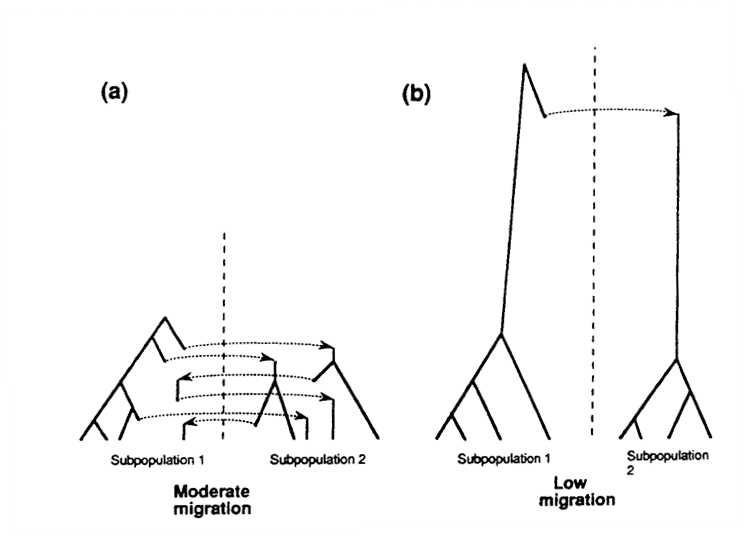
\includegraphics{coalescent-process.images/image6.png}
    \caption{图 6}
\end{figure}

图 6 (a)大小为 8 的一个样本的系谱图举例, 分别来自 2 个亚群体, 每个亚群体 4 个, 迁移率适度高.
每个迁移事件用一条带箭头的点状线表示箭头代表一个个体迁移者的实际移动方向. 在这种情况下, 这两个亚群体应该有相对小的分化.
(b)低迁移率的系谱举例. 在这个系谱图上只有一个迁移事件. 来自同一个亚群体内部的等位基因比来自不同亚群体的等位基因更相似.

这些系谱也可以被解释成含有不同的所选等位基因的配子的系谱. 亚群体 1 代表含有 \textbf{S} 基因的配子库, 亚群体 1 代表含有
\textbf{F} 基因的配子库. 在这种情况下, 带箭头的点状线代表把一个 \textbf{F} 基因变成一个 \textbf{S} 基因的突变,
反之亦然. 如果在所选等位基因间的突变率是高的, 含有不同等位基因的序列将不会比含有相同等位基因的序列有更多差异. 如果
\textbf{S} 和 \textbf{F} 之间的突变率是低的, 那么含有 \textbf{S} 的配子和含有 \textbf{F}
的配子之间将是相对分离的. 这些系谱也可以代表和一个选定的基因座连锁的一个位点的系谱. 在这种情况下,
带箭头的点状线代表所选等位基因之间的突变率和/或和所选基因座连锁的位点间的重组事件.

\begin{figure}
    \centering
    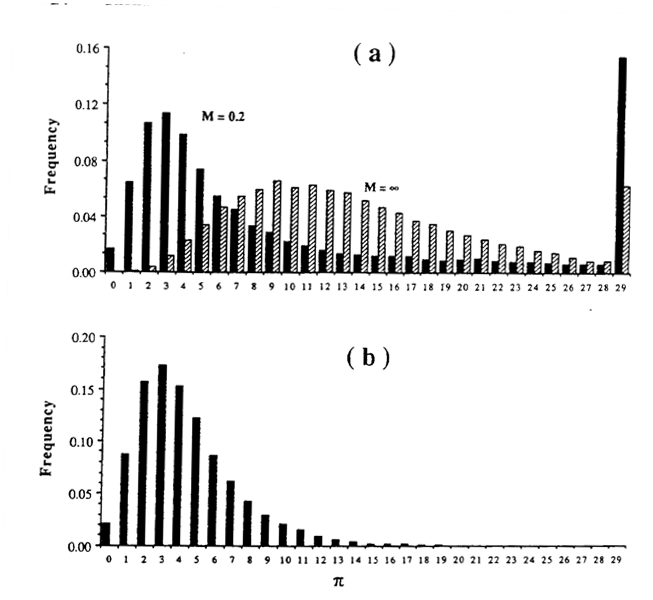
\includegraphics{coalescent-process.images/image7.png}
    \caption{图 7}
\end{figure}

图 7(a) $\uppi$ 的分布, $\uppi$ 为取自同一个亚群体的大小为 10 的样本中等位基因间差异的平均对数. 群体由三个亚种群组成,
每一个都是大小为二倍体 $N$, $\uptheta =4Nmu =5$, 其中 $M=4Nm=0.2$ (实心条) 和 $M=\mathrm{\infty}$ (斜纹条) .
两个分布的平均值都大约是 15. (b)对于一个单独的的随机交配群体, 相同数量的分布 $\uptheta =4N\upmu =5$.
注意和(a)中低迁移率的情况的相似性.

\section{平衡选择}

Kaplan 等已经给出了怎样在有某种形式的选择模型下分析溯祖过程.
他们主要关注一个特定核苷酸位点上含有两个等位基因多态性的平衡选择的情况, 这个特定的核苷酸位点为 ``选择位点''.
假设在每一次复制中两个选择等位基因之间的循环突变率为 $\upnu$, 这两个等位基因用 \textbf{F} 和 \textbf{S} 表示.
分析导致这个问题: 对于和选择位点完全连锁的位点的系谱和一个独立于任何选择之外的中性位点的系谱有怎样的不同?当选择弱,
并且在选择位点的基因频率可以相当大地漂移时, 花些力气可以得到数值结果 (Darden 等 1989). 当选择很强且不变时,
结果相当简单, 前提是选择基因 \textbf{S} 和 \textbf{F} 的频率保持恒定.

强的和保持不变的选择情况下, 样本基因的溯祖过程和细分的群体模型的溯祖过程相似, 除了迁移不再是均衡的. 如果 \textbf{S} 和
\textbf{F} 的频率分别为 $p$ 和 $q$, 然后可以考虑群体被再分成大小为 $2Np$ 和 $2Nq$ 的两个亚群体. 突变担当迁移的角色.
每一代, 平均 $2Nq\upnu$ 个 \textbf{F} 基因突变 (迁移) 成为 \textbf{S} 基因 (亚群体) , $2Np\upnu$
个向另一个方向突变. 这意味着每一代中一定比例的 \textbf{S} 基因, $2Nq\upnu/2Np$, 大约是上一代 \textbf{F}
基因的后代. 换句话说, 一代中的一个 \textbf{S} 基因的亲本是 \textbf{F} 基因的概率是 $q\upnu/p$. 如果考虑 $n_{1}$
个 \textbf{S} 基因, 其中一个的亲本是 \textbf{F} 基因的概率 $P_{\text{SF}}$ 大约是:

\begin{equation*}
    P_{\text{SF}}=n_{1}\frac{q\upnu}{p}
\end{equation*}

同样的, $n_{2}$ 个 \textbf{F} 基因, 其中一个的亲本是 \textbf{S} 基因的概率 $P_{\text{FS}}$ 大约是: \newline

\begin{equation*}
    P_{\text{FS}}=n_{2}\frac{p\upnu}{q}
\end{equation*}

量 $p\upnu/q$ 和 $q\upnu/p$ 类似于细分群体模型(subdivided population model)中的迁移. 在这种情况下, ``迁移''
不再是对称的, 并且两个 ``细分群体'' 的大小不相等.

溯祖事件的概率是每个细分群体的基因大小的函数. 比如说, 两个 \textbf{S} 配子在上一代有一个共同祖先的概率大约是 $1/2Np$,
对于 \textbf{F} 配子来说, 相应的是 $1/2Nq$. 更普遍地, $n_{1}$ 个 \textbf{S}
基因中的任意两个在前一代有共同祖先的概率 $P_{\text{CA},\mathrm{S}}$ 是:

\begin{equation*}
    P_{\text{CA},\text{S}}=\frac{\binom{n_1}{2}}{2Np}
\end{equation*}

同样的, 对于 $n_{2}$ 个 \textbf{F} 基因, 其中任意两个在前一代有共同祖先的概率
$\text{P}_{\text{CA},\text{F}}$ 是:

\begin{equation*}
    P_{\text{CA},\text{F}}=\frac{\binom{n_2}{2}}{2Nq}
\end{equation*}

包含不同基因型 \textbf{F} 和 \textbf{S} 的共同祖先事件要求一个突变和在同一代的一个共同祖先事件.
在低突变率和大的群体大小情况下, 这是不太可能的, 我们忽略这种概率.

对于一个含有 $n_{1}$ 个 \textbf{S} 基因和 n$_{\text{2}}$ 个 \textbf{F} 基因的样本, 把这个过程的要素放在一起,
每一代事件的总比率是:

\begin{equation*}
    P_{\text{tot}} = P_{\text{CA},\text{S}} + P_{\text{CA},\text{F}} + P_{\text{FS}} + P_{\text{SF}}
\end{equation*}

因此, 回溯到某个事件的时间是指数分布的, 有平均值 $1/P_{\text{tot}}$. 假设一个事件发生了,
概率时间这个事件发生的比率除以总事件的比率. 比如说, 我们沿着世系向前追溯,
第一个事件是一个 \textbf{S} 基因变成一个 \textbf{F} 基因的概率是 $P_{\text{SF}}/P_{\text{tot}}$,
在这种情况下, 我们的样本的祖先在第一个事件发生的那一代应该包含 $n_{1}-1$ 个 \textbf{S} 基因和 $n_{2}+1$
个 \textbf{F} 基因. 最终, 结合其他模型, 溯祖事件将会导致整个样本的一个共同祖先.

溯祖过程的分析显示, 如果 \textbf{S} 和 \textbf{F} 间的突变率很小,
一个随机的 \textbf{S} 和一个随机的 \textbf{F} 找到一个共同祖先的平均时间是很大的, 如我们和迁移模型类比所预料到的. Kaplan
等 (1988) 也表明, 如果随机选取 $n$ 个基因, 不考虑哪个基因出现选择位点, 如果 $4N\upnu$ 小,
样本系谱上的总时间比在严格中性模型下要大得多. 如果 $4N\upnu$ 大, 到共同祖先的平均时间本质上不受选择的影响. 图 6b
显示的系谱举例展示了一个典型的低突变率下的系谱. 细分模型和平衡模型之间的一个不同是,
地理细分情况下所有位点应该以相同方式受影响, 选择情况下, 只有和选择位点紧密连锁的位点显示大的系谱.

Hudson 和 Kaplan (1988) 表明了之前叙述的在选择模型中加入重组是直截了当的. 考虑一个基因座的溯祖过程,
可能是和一个选择位点连锁的一个核苷酸位点. 用 $r$ 代表每一代中某基因座, 称为 \textit{A} 基因座, 和选择位点的重组率.
由于重组, \textit{A} 基因座样本的系谱不同于选择位点的系谱. 但是系谱过程很相似.
考虑一个选择位点含有 \textbf{S} 基因的配子样本. 我们称之为含有 \textbf{S} 的配子. 配子的亲本 (在 \textit{A} 位置)
很可能也和 \textbf{S} 基因连锁, 但是因为产生我们的样本配子的过程中可能发生突变或重组,
亲本的 \textit{A} 位置可能和一个 \textbf{F} 基因连锁. Hudson 和 Kaplan 显示了每一代中这种改变
(从与 \textbf{S} 连锁到与 \textbf{F} 连锁) 的概率是 $q\upnu/p+2pqr/p=(\upnu+pr)q/p$. 同样的,
一个含有 \textbf{S} 的配子的 A 基因座的亲本是一个含有 \textbf{S} 的配子的概率是 $(\upnu+pr)q/p$. 因此,
对于连锁位点的溯祖过程和完全连锁的位点一样, 除了在某些情况下用 $\upnu+pr$ 代替 $\upnu$, 另一些情况下用 $\upnu+qr$ 代替 $nu
$. 假设 $p$, $r$, $\upnu$ 和 $N$ 保持不变, 事件之间时间是指数分布的. 事件之间的平均时间和不同可能的改变的相对概率依赖于
$2N\upnu$, $2Nr$ 和 $p$.

如我们所料, 如果一个位点和选择位点是紧密连锁的 ($2Nr$ 小) , 并且 $2Nnu$ 小,
含有 \textbf{S} 的配子的位点和含有 \textbf{F} 的配子的位点到达共同祖先的时间的期望比严格中性的情况更大. 换句话说,
当比较含有不同选择等位基因的序列时, 和选择位点紧密连锁的位点差异将会相对高. 不紧密的连锁位点受平衡选择的影响相对小. 因此,
在含有不同等位基因的序列比较中, 预计在序列上选择位点的中央有一个差异的峰值.

选择性保留 (selectively maintained) 的单核苷酸位点多态性能在连锁位点上显著提高中性多态性的水平,
使之能在样本中可以发现. 因此, 存在寻找异乎寻常高的多态性水平的染色体区域来发现选择性保留的变异的潜在可能性.
这个方法的一个问题是位点和位点之间或区域和区域之间的选择约束条件是不同的,
所以特定区域的高水平多态性可能可以用降低的约束条件假设似乎有道理地解释. 但是,
可以比较近缘物种的序列来检验这个降低约束条件的假说. 这是因为在中性模型下, 约束条件的水平不仅仅决定物种内多态性的预期水平,
还决定了物种间的差异水平. 因此, 如果在物种内一个区域有相对高的多态性水平是因为约束条件的降低,
应该会呈现出物种间相对高的差异水平. 换句话说, 在考察染色体组的不同区域时可以看到种间差异水平和多态性水平的强相关性.

平衡选择维持的多态性存在会引起从这种种间差异和种内多态性相关的形式的大的偏离. 平衡选择维持的多态性,
从两个物种分化时开始发生的, 对区分这两个种的中性突变的积累没有影响, 如第 2 小节讨论的.
在种间分化前发生的和从起源起连续维持的平衡多态性可以导致连锁位点的物种间中性差异比非连锁位点的大.
两物种种间差异的时间减小了影响的大小. 因此, 依赖于什么时候平衡多态性发生, 平衡选择可能对种间差异有很小的影响,
但是如之前所讨论的, 将会显著提高种内紧密连锁位点的中性多态性水平.

一个中性统计学试验设计出来用于检验种间差异和种内多态性是否显示了中性条件下预期的一致性 (Hudson 等 1987; Kreitman 和
Augeade 1986). 这个测验在 \textit{Drosophila melanogaster} 和 \textit{D.
sechellia} 的乙醇脱氢酶区域的数据的应用上导致了对中性的否决.
数据与中性预期的背离和 \textit{Adh} 编码区平衡多态性的存在相一致.
有大量独立证据证明了选择在 \textit{Adh} 的 \textbf{F}/\textbf{S} 多态性的维持中的重要性 (Oakeshot 等 1982).

如果数据与中性模型预期的背离归因于作用在 \textit{Adh} 的 \textbf{F}/\textbf{S} 蛋白多态性上的平衡选择,
之前描述的有平衡选择和重组的模型是合适的.
我们应该可以从数量上预期那些选择导致的大的系谱所引起的紧密连锁位点的种间差异的增加水平.
\textit{Adh} 的 \textbf{F}/\textbf{S} 多态性是由 \textit{Adh} 基因的 192 号的一个核苷酸的多态性产生的.
在选择模型下预测和 \textit{Adh} 基因的 192 号连锁的位点的多态性水平, 必须给参数指定一个值. 需要的参数有: $p$,
\textbf{S} 基因的频率;$2N\upnu$, 其中 $\upnu$ 是被选择基因间的突变率;$\uptheta$
连锁位点上每个碱基对的中性突变率;$R=4Nr$, 其中 $r$ 是每个碱基对的重组率. 对于所有这些参数,
预先可知的信息允许我们指定这些参数的近似值, 然后比较序列之间差异的预期水平和 Kreitman 观察的序列数据水平 (1983) .

为了展示观察的和预测的序列间差异, 作为沿着序列的位置函数, 采用一个滑动窗口的方法. 在这个方法中,
一个窗口沿着直链序列顺序地滑动. 在窗口的每一个位置, 多态性水平由窗口中相邻位点的集合表示. 用这个方法,
作为核苷酸位置函数的多态性可以被表示出来. 多态性水平用窗口中序列之间的碱基对差异的平均数来衡量.
改变窗口的宽度来加入蛋白编码的约束条件, 以使沉默的改变的数量可能保持恒定. 对于 \textbf{F}/\textbf{S} 的比较, 已用除 $R$
以外的参数的预先估算得到了一个合理的观察和预期的拟合性. 我们对 $R$ 的预先估计是 24.0, 但是最好的拟合性是用 $R=4.0$
得到. 然而, 含有 \textbf{S} 基因的序列间的差异的观察值和预测值之间有相当大的差异. 有兴趣的读者可以参考 Hudson 和
Kaplan(1988)得知更多细节.

Hudson 和 Kaplan (1988) 的预测是基于所有位点不影响 \textit{Adh} 酶的氨基酸序列的假设之上的,
这些位点是非编码位点或是同义突变位点, 有相同的中性突变率参数 $\uptheta$. 也假设这些位点上有 0、1 或 2
个同义核苷酸改变是可能的, 分别有中性突变参数 0, $\uptheta /3$, $2 \uptheta /3$. 有了这些假设, 只需要一个中性突变参数. 然而,
似乎合理的是约束条件水平, 从此时起是中性突变参数, 对于所有的非氨基酸改变位点不再是相同的.

更详细的分析可能用近缘种 \textit{Drosophila simulans} 的序列数据去估算不同位点的突变参数.
我们可以按照如下方法用物种间的数据估算突变参数. 让我们假定位点间的中性突变参数不同, 用参数 $\uptheta_{i}$ 表示位点 $i$
的中性突变参数. 用 $t$ 代表两个序列自共同祖先以来的平均时间, 这两个序列分别来自 \textit{D. melanogaster} 和
\textit{D. simulans}. 如果 $\uptheta_{i}t$ 足够小, 这两个序列在 $i$ 位点不同的概率大约是 $\uptheta_{i}t$. 因此,
一个由 $l$ 个核苷酸组成的小区域的 $\uptheta$ 的平均值, 可以用 $d/tl$ 来估算, 其中 $d$ 是两个物种在这 $l$
个核苷酸区域的不同位点数目. 这种估算有如下应用.

一个窗口 (同样用于展示观察到的和预测的种内多态性) 沿着一对线性序列滑动, 这两个序列一个来自 \textit{D.
    melanogaster} 另一个来自 \textit{D. simulans}. 在窗口的每一个位置, 窗口中的序列间差异的数目被数出来, 并且用 $t$
和窗口宽度的乘积去除. 这个量作为窗口中间位点的 $\uptheta$ 的估算. 这显然是一个平滑过程,
这个过程指定了某个位点由周围位点变异的积累所决定的 $\uptheta$ 值. 选取 $t$ 来产生一个好的拟合性,
因此而给出一个符合观察值的多态性平均水平. 手上有这些 $\uptheta_{i}$, 就可以预测和选择位点连锁的任何位点集合的多态性.

把这个方法用于 Kreitman (1983) 的多态性数据, 增补额外的 \textit{D. melanogaster} 的 5${\prime}$ 和
3${\prime}$ 数据以及 \textit{D. simulans} 的一个序列, 观察的和预测的多态性水平如图 8 所示. 假设完全中性,
整体忽略 \textbf{F}/\textbf{S} 多态性, 两个取样序列在一个区域内差异的预期数目是这个区域内位点的 $\uptheta _{i}$ 之和.
这个预测如图 8a 所示. 因为 $\uptheta _{i}$ 和两物种间的差异是成比例的, 图 8 所示的预测的多态性水平与 \textit{D.
    melanogaster} 和 \textit{D. simulans} 之间的差异水平是成比例的. 看起来有较高和较低约束条件的区域. 特别注意的是
5${\prime}$ 侧翼区低的预测多态性水平和低的观察多态性水平, 在图 8 中数目大约是 400-450.
也要注意 \textit{Adh} 的第三个编码外显子的沉默位点预测有一个相对高的多态性水平. 这归因于这些位点的物种间的相对高水平的差异.
但是观察到的这些位点的多态性水平比预测的更高. 如果假设 192 号 \textbf{F}/\textbf{S} 位点多态性是平衡的,
高水平的多态性能够很容易地解释, 如图 8b 所示. 产生这个拟合性的重组参数是 $R=12.0$, 只比 Hudson 和
Kaplan (1988)给出的预先估算小了 2. 预期和观察的 \textbf{S} 基因间的多态性水平如图 9 所示. 观察和预测的拟合性如图 9
所示, 用物种间估算出的 $\uptheta _{i}$ 得到, 这个拟合性比 Hudson 和 Kaplan 用恒定的得到的拟合性要显著的好.
\textbf{F} 基因之间观察到的和预测的差异都很低, 没有显示出来.

同时使用物种内多态性和物种间差异的分析可能对检测中性选择作用是特别有效的,
这里指出的平衡和将在下一章中叙述的有利突变的固定都有效. 对于选择是否在可溶酶基因座的电泳可检测的多态性的维持中有重要作用,
群体遗传学已经争论了 20 年. 如果像 \textit{D. melanogaster} 这样详细的位点能被发现的话, 看起来还会有有意义的进展.
有了现代的聚合酶链式反应, 这样的任务看起来不再是不可能的. 在很多情况下, 选择已经强烈显示来,
比如 \textit{Fundulus} 中的 \textit{Ldh}(Powers 等 1983), \textit{Mytilis} 中的 \textit{Lap}(Hilbish 和
Koehn1985), \textit{Tigriopus} 中的 \textit{Gpt}(Burton 和 Feldman1983), \textit{D.
    melanogaster} 中的 \textit{Gpdh} (Barnese 和 Laurie-Ahlberg 1986 ;Oakeshott 等 1984), 和 Koehn 等 (1983)
和 Zera 等 (1985) 描述的其他一些可能提供了好的测验例子, 如果序列能得到的话.

Hudson 等 (1987) 的测验对于检测选择的统计学能力还有待研究. 图 8 和 9
所示的观察的和预测的曲线的拟合度好坏的度量也有待研究.

\begin{figure}
    \centering
    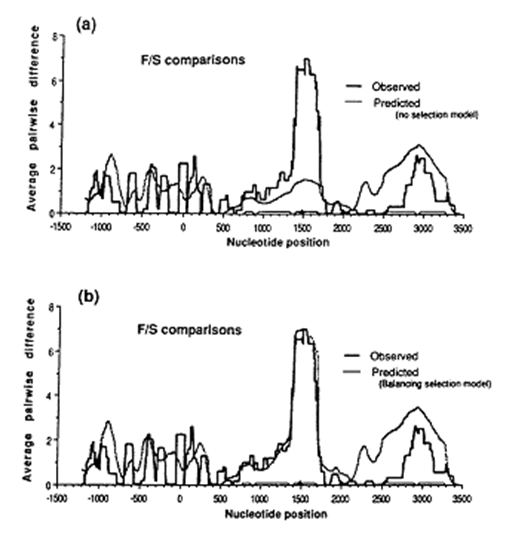
\includegraphics{coalescent-process.images/image8.png}
    \caption{图 8}
\end{figure}

图 8 在一个 ``滑动窗口'' 中, 含有 F 的序列和含有 \textbf{S} 的序列之间差异的观察值和预测值相对于核苷酸的位置作图. Adh
的编码外显子和重复基因座在位置轴上用低的矩形表示出来. \textbf{F}/\textbf{S} 的多态性位点, \textit{Adh} 的 192
号密码子, 用黑色三角形表示. 窗口的宽度经过调整, 使得窗口中总有 300 个可能的同义突变位点.

基于没有平衡选择的严格中性模型的预测曲线. \textit{D. melanogaster} 和 \textit{D. simulans}
之间的物种间序列比较被用于确定文中所述的每个位点的 $\uptheta$. 中性模型下, 成对的差异 (pairwise difference)
简单地就是窗口中这些位点的 $\uptheta$ 之和. 假设 $t$ 的值是 5, $t$ 是以 $2N$ 代为单位衡量的物种分化时间.
(b)预测曲线是基于平衡选择模型的, 参数值为: $\beta = 0.001$, $R = 4Nr = 12.0$, $t=5$, $p=0.7$
(见正文中对这些参数的解释).

\begin{figure}
    \centering
    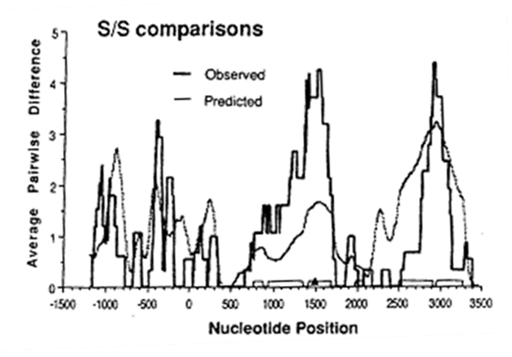
\includegraphics{coalescent-process.images/image9.png}
    \caption{图 9}
\end{figure}

图 9 一个滑动窗口中, 含有 \textbf{S} 的配子间差异的预测值 (平衡选择模型下) 和观察值相对于核苷酸位置作图. 所有参数和图
8 中一样.

\section{搭乘效应}

用溯祖方法, Kaplan 等 (1989) 分析了一个模型, 其中罕见的有利突变横扫整个群体.
他们再分析了连锁位点上优势变异的选择性突变的搭乘效应(Maynard Smith 和 Haigh1974). 这个过程很像平衡选择模型,
除了选择基因的频率随时间改变, 因而溯祖事件的概率, 和其他事件一样, 随时间改变. 因此, 事件之间的时间间隔不再是指数分布的.
如果有利基因的频率能用一个确定的函数近似表示, 结果可以用直接的数值方法得到. 用这种方法,
可以估算连锁的核苷酸位点上的中性变异被一个有利突变的快速固定减少了多少.

图 10 显示了一个系谱图, 举例证明了一个基因树的形状在一个近期的搭乘事件后与平衡中性突变模型的系谱 (图
\ref{fig:1}) 相比有多不同. 图 10 中的大多数包含了没有向下分支出一个单独取样配子的世系. 用这个系谱模式,
一个 ``星形'' 系谱, 多数中性突变会导致多态性, 在每个多态性位点,
突变核苷酸只被替换一次并且没突变的核苷酸在所有子代序列中出现. 就是说, 大多数核苷酸位点将会有一个低频率等位基因,
在样本中出现一次或者两次, 和一个非常高频的等位基因. 没有一个特定的配子会带有大量稀有的突变,
但是可以期望有一个高度差异的世系. 这个主要是低频多态性的模式特有的是一个近期重度的瓶颈之后的群体,
这个瓶颈导致了大多数世系在一个相对短的时期内追溯到共同祖先 (coalescent) . 和搭乘模型相比, 一个群体瓶颈之后,
所有基因座可以预计有与众不同的系谱. 多态性的频谱可以证明是核苷酸多态性的一个特别有用的特征.

\begin{figure}
    \centering
    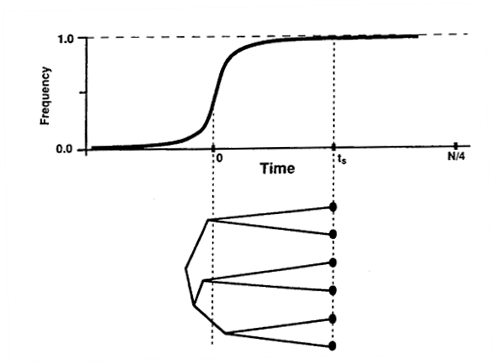
\includegraphics{coalescent-process.images/image10.png}
    \caption{当一个选择上有利的突变刚刚固定时的一个含 6 个等位基因的样本的系谱图举例.
        黑体的曲线显示了有利突变的频率作为时间的函数. 样本在 \(t_{\mathrm{s}}\)
        时刻的系谱在函数上叠加表示出来. 例子中没有描述重组. 如果
        \(t_{\mathrm{s}}\) 显著小于 \(N\), 多数溯祖事件会发生在接近 0 时刻处.
        在这种情况下, 和没有选择的系谱相比, 系谱的总体大小将会是小的,
    因此将会有相对少的变异. 同样, 系谱的形状和中性平衡的系谱不同}
\end{figure}

\section{结语}

聚焦溯祖过程是在多样的情况下考虑样本性质的一种有用方法. 我们可以看到, 在多样的情况下, 能够相对容易地描述溯祖过程.
加上上一章中描述的情况, 溯祖过程已经被用于检验有基因转换的多基因家族中基因的变异 (Kaplan 和
Hudson1987;Watterson1986b) , 以及转座子家族 (Hudson 和 Kaplan1986b) 、高度重复分散元件, 如 ALU (Kaplan 和
Hudson1987) . 在这里叙述的很多分析, 系谱的总体复杂性简化成一或两个统计量, 即系谱有多大, 或者等效地,
预计有多少突变在系谱上发生. 某些情况下, 也可以问取自一个亚群体或某个选择性存在的基因类的样本的系谱有多大,
或者不同类别或等位基因有多少核苷酸分歧. (对所有含有特定电泳等位基因序列二次取样也能得到系谱大小: Hudson 和
Kaplan1986a) . 值得注意的是这些性质常常从经典方法得到, 没有准确提及样本的系谱, 用一代递归或者扩散方法(Watterson
1989a). 但是系谱方法直观、清楚, 提供了一个普遍的方法来得到结果和设想很多模式下预期的变异样式. 对于没有重组的的区域,
系谱是概括复杂信息的有效途径, 经验的和理论的, 如 Avise 等 (1987) 和 Cann 等 (1987) 在线粒体变异方面的工作所例证的.

利用样本系谱实际数据的方法, 与仅仅用 \textit{S} 相反, 可能在某些情况下特别有效. 引人注目的是 Golding(1987; Golding 等
1986)和 Iizuka(1989)的工作, 为了查明选择而检验了系谱上不同种类的突变的分布. Slatkin(1989)和 Slatkin 和
Maddison(1989)已经开始探索用详细的系谱信息推断地理结构的方法.
用无根树形式的详细系谱信息对突变参数的估算已经被仔细检查过(Strobeck 1983). 样本等位基因的系谱上有大量的信息.
探究这些信息的额外的方法是需要的.

对于重组水平高的区域, 详细的系谱也许不可能有任何可靠性的推断. 对于核基因, 相距几百碱基对的位点的系谱可以显著不同.
我们推理一个几百个碱基对的片段的系谱的能力是非常有限的.
中等长度序列的样本的系谱常常会是一个难以置信复杂的世系、溯祖过程和断裂的网络.

尽管至少中等水平的重组下某种系谱信息可能存在 (Golding 1987), 但当分析高度重组区域的数据时概要的统计量可能是非常重要的,
而不是详细的系谱重建. 可能有用的量包括多态性水平 (用 $S$ 或平均差异对数来衡量) , 变异频谱,
和不同种类的变异之间的这些量的对比, 比如沉默的和编码的、插入/缺失和替换或者和不同电泳等位基因相关的变异. Sawyer
等(1987)用了这样一种方法. 物种内可见的模式和物种间观察到的模式之间的比较将会提供大量信息(Kreitman 1987),
建议平衡选择位点、搭乘事件, 或者发生了突变率或约束条件的剧烈改变.
十或十五个有酶多态性的位点可能可以用和 \textit{Adh} 相同的方式有效地检测. 对于在各种模型下得到这些量的一些统计学性质,
溯祖过程是有用的. 毕竟应用于单个位点系谱的无重组分析忽略了有多少重组发生. (如果每一个核苷酸位点的突变率足够低,
无限位点或无限等位基因模型对于单核苷酸位点仍是准确的. 对于高突变率, 可能需要有限等位基因模型. ) 但是,
充分考虑到连锁位点的非独立性, 可能证明了用任何方法都非常困难, 不论经典的或溯祖的. 处于这个原因,
基于溯祖过程的模拟将会在统计学方法、试验和评估的研究中扮演重要的角色.

考虑无重组模型的惯例, 和蒙特卡洛 (Monte Carlo) 模拟一起, 可能是分析种内分子变异的方法发展的重要路线.
基于有重组溯祖过程的模拟是重要的秩序, 比执行过时的在计算机里重现整个世代的相似模拟和费时的取样产生连续世代的大数量更快捷.
模拟的方法可以直接地合并, 同时地, 重组, 地理结构, 群体大小变异和不平衡情况, 还有环形染色体组和选择形式, 和各种突变方案.
这种模拟将在建立估计量的置信区间, 统计试验的显著点, 和依靠各种可供选择的模型的试验的效力上发挥作用.

尽管分析来着重组 DNA 的数据有困难, 但是这些数据在某些情况下可能是首选的. 考虑一个整个分子有一个单独系谱的线粒体样本,
因为没有重组. 因为线粒体基因组中含有大量位点, 可以希望能准确推断系谱.
但是得到的系谱是对控制所取样群体的分子进化的随机过程的单一认识. 从一次观察中得到的对于随机过程推断的自信是有限的.
对于核基因组, 我们常常不能准确推断系谱, 因为不同程度的统计学独立性. 每一个片段将会经历与亚群体和群体大小一样的历史.
如果有这种能帮助我们估算参数或检验假说的样本统计学性质, 积累不同位点的信息的可能性使得核基因组潜在地能提供更多信息.
比如说估算迁移率和突变参数, 用核基因可能更精确.
用于检验 \textit{Adh} 内部或附近变异的分析类型可能不能仅仅用线粒体数据实现. 但是可以用 Hudson 等 (1978) 的检验, 用
mtDNA 作为一个基因座, 核基因作为另一个基因座.

中性模型和恒定选择系数的某种模型下预期的系谱在一定程度上已经描绘出来. 一类不能预测系谱的重要的模型是随机环境模型. 重要的是,
是否这些模型预测的系谱进而中性模型预测的系谱很不相同.

群体内的 DNA 多态性已经从它们应对关于群体内遗传变异的长期问题的有效性上显示出来. 随着更多数据被收集,
很明显系谱分析将会参与理解已经显露出的那些模式.

\section{名词与符号}

% no nomenclature title
\renewcommand{\nomname}{}

% nomenclature groups
\renewcommand\nomgroup[1]{%
    \item[\bfseries
        \ifstrequal{#1}{A}{缩写}{%
            \ifstrequal{#1}{N}{名词}{%
                \ifstrequal{#1}{F}{函数}{%
                    \ifstrequal{#1}{S}{符号}{}}}}%
    ]
}
                
\nomenclature[A]{DNA}{Deoxyribonucleic acid, 脱氧核糖核酸}
\nomenclature[A]{MRCA}{Most Recent Common Ancestor, 最近共同祖先}
\nomenclature[A]{bp}{base pair, 碱基对}
\nomenclature[A]{W--F model}{Wright--Fisher model, W--F 模型}
                                                        	      	
\nomenclature[N]{Pedigree}{家谱}
\nomenclature[N]{Lineage}{世系}
\nomenclature[N]{Genealogy}{系谱}
\nomenclature[N]{Sample}{样本}
\nomenclature[N]{Gene tree}{基因树}
\nomenclature[N]{Polymorphism}{多态性}
\nomenclature[N]{Homologous sequences}{同源序列}
\nomenclature[N]{Coalescent process}{溯祖过程}
\nomenclature[N]{Allele}{等位基因}
\nomenclature[N]{Variation}{变异}
\nomenclature[N]{Infinite-site model}{无限位点模型}
\nomenclature[N]{Infinite allele model}{无限等位基因模型}
\nomenclature[N]{Equation}{方程}
\nomenclature[N]{Demographics}{人口统计学}
\nomenclature[N]{Sampled allele}{样本等位基因}
\nomenclature[N]{Stochastic precess}{随机过程}
\nomenclature[N]{Hitchhiking}{搭乘效应}
                                                        	      	
\nomenclature[F, 01]{$E()$}{Expected value, 期望值}
\nomenclature[F, 02]{$\text{Var}()$}{Variance of expected value, 期望值的方差}
                                                        	      	
\nomenclature[S, 01]{$\upmu$}{The mean number of mutations, 突变数的平均值}
\nomenclature[S, 02]{$t$}{The number of generations since the MRCA of two sampled homologous sequences, 从 MRCA 到两个抽样的同源序列的世代数}
\nomenclature[S, 03]{$S$}{The number of mutations that have occurred in the descent to the two descendent sequences, 向下到这两个后代的序列过程中产生的突变数}
\nomenclature[S, 04]{$T_{\text{tot}}$}{The sum of the lengths of the branches of the genealogy of a sample, 一个样本的系谱中所有分支长度的总和}
                                                        	      	
\printnomenclature
                                                        	      	
\end{document}
